\section{Resoconto delle attività di verifica}

In questa sezione vengono inserite tutte le misurazioni delle metriche trovate dal gruppo \gruppo.
Il team si impegna a garantire almeno il soddisfacimento del range di accettazione per ogni metrica.

Per quanto riguarda le misurazioni può essere calcolato un risultato singolo, se la metrica si riferisce ad una caratteristica singola, oppure può essere calcolato un risultato massimo, ovvero una metrica che si riferisce a più componenti, ad esempio le classi. In tal caso verrà presa la misurazione peggiore e confrontata con i valori scelti dal team precedentemente.

Alcune metriche, infine, sono state misurate più volte nel tempo e per queste verrà illustrato un diagramma cartesiano, in cui: l'asse delle ascisse rappresenterà in giorni la durata del periodo fino alla consegna, mentre l'asse delle ordinate rappresenterà i valori assunti al momento delle misurazioni. \\
Verranno comunque riportati i risultati finali di tali metriche nell'apposita tabella.


\subsection{Revisione dei Requisiti}
In questa sezione vengono inseriti i risultati relativi al periodo di Revisione dei Requisiti e le metriche relative ad esso.

\subsubsection{Analisi statica dei documenti}
L'analisi statica dei documenti è stata fatta mediante \termine{Walkthrough} ed ha portato all'individuazione di alcuni errori. Tra gli errori individuati quelli più frequenti sono stati:
		\begin{itemize}
			\item Errori nei concetti esposti.
			\item Aggettivi o verbi utilizzati in modo scorretto.
			\item Periodi troppo lunghi o complessi da capire ed interpretare.
		\end{itemize}

\subsubsection{Esiti verifiche automatizzate}
		
\paragraph{Indice di Gulpease}

\begin{table}[h]
	\begin{center}
		\begin{tabular}{|c|c|c|c|}
			\hline
			\textbf{Documento}	& \textbf{Risultato} & \textbf{Esito} & \textbf{Valore} \\
			\hline
		 \termine{Analisi} dei Requisiti v1.0.0 & 90 & Superato & Ottimale	\\
			\hline
			Glossario v1.0.0 & 56 & Superato & Ottimale	\\
			\hline
			Norme di Progetto v1.0.0 & 47 & Superato & Accettabile \\
			\hline
			Piano di Progetto v1.0.0 & 48 & Superato & Accettabile\\
			\hline
			Piano di Qualifica v1.0.0	& 48 & Superato & Accettabile\\
			\hline
			Studio di Fattibilità v1.0.0	& 47 & Superato & Accettabile\\
			\hline
			Verbale\_Esterno\_1\_20161223 v1.0.0	& 51 & Superato & Ottimale	\\
			\hline
		\end{tabular}
	\end{center}
	\caption{RR - Risultato indice di Gulpease}
\end{table}

\subsubsection{Soddisfacimento metriche}

\paragraph{Qualità di processo}
\begin{longtable}{|>{\centering}m{5cm}|c|c|c|c|c|}
\hline
\textbf{Metrica} & \textbf{Unità di misura} & \textbf{Risultato} & \textbf{Risultato Massimo} & \textbf{Esito} & \textbf{Valore}\\
\hline
\endhead

\emph{Schedule Variance} & {Attività} & \textcolor{Green}{0} & / & Superato & Ottimale\\ \hline
\emph{Budget Variance} & {Euro} & \textcolor{Green}{15} & / & Superato & Ottimale \\ \hline
\emph{Rischi non preventivati} & {Rischi} & \textcolor{Green}{0} & / & Superato & Ottimale\\ \hline
\emph{Ottimalità delle misurazioni} & {Percentuale} & \textcolor{Green}{0.6} & / & Superato & Ottimale \\ \hline
\emph{Rischi non preventivati} & {Rischi} & \textcolor{Green}{0} & / & Superato & Ottimale\\ \hline
%\emph{Efficienza di gestione dei rischi} & {Giorni} & \textcolor{Orange}{21.3} & $\geq 20$ & $\geq 60$\\ \hline
%\emph{Requisiti obbligatori soddisfatti} & {Percentuale} & \textcolor{Green}{100} & $100$ & $100$\\ \hline
%\emph{Livello di stabilità-SDK} & {Percentuale} & / &\textcolor{Green}{1} & Accettabile\\ \hline
%\emph{Livello di stabilità-Applicazione} & {Percentuale} & / &\textcolor{Green}{1} & Accettabile\\ \hline
%\emph{Astrattezza-SDK} & {Percentuale} & / &\textcolor{Green}{0.8} & Accettabile\\ \hline
%\emph{Astrattezza-Applicazione} & {Percentuale} & / &\textcolor{Green}{0.5} & Ottimale\\ \hline
%\emph{Distanza dalla sequenza principale-SDK} & {Percentuale} & / &\textcolor{Green}{1} & Accettabile\\ \hline
%\emph{Distanza dalla sequenza principale-Applicazione} & {Percentuale} & / &\textcolor{Green}{0.7} & Accettabile\\ \hline
%\emph{Numero di metodi per classe} & {Metodi} & / &\textcolor{Green}{11} & Accettabile\\ \hline
%\emph{Numero di attributi per classe} & {Attributi} & / &\textcolor{Green}{7} & Ottimale\\ \hline
%\emph{Numero di parametri per metodo} & {Parametri} & / &\textcolor{Green}{7} & Ottimale\\ \hline
%\emph{Produttività di codifica} & {Linee} & \textcolor{Orange}{9.1} & $\geq 3$ & $\geq 10$\\ \hline
%\emph{Complessità Ciclomatica media} & {Cammini} & \textcolor{Green}{0} & $1 - 15$ & $1 - 10$\\ \hline
%\emph{Livelli di annidamento medi} & {Chiamate} & \textcolor{Green}{1} & $1 - 6$ & $1 - 3$\\ \hline
%\emph{Linee di codice per linee di commento} & {Percentuale} & \textcolor{Green}{31} & $\geq 25$ & $\geq 30$\\ \hline
%\emph{Variabili inutilizzate} & {Variabili} & \textcolor{Green}{0} & $0$ & $0$\\ \hline
%\emph{Dipendenze} & {Chiamate require} & \textcolor{Green}{2.2} & $0 - 10$ & $0 - 5$\\ \hline
%\emph{Halstead Difficulty media} & {Percentuale} & \textcolor{Green}{0} & $0 - 25$ & $0 - 15$\\ \hline
%\emph{Halstead Volume media} & {Percentuale} & \textcolor{Green}{20} & $20 - 1500$ & $20 - 1000$\\ \hline
%\emph{Halstead Effort media} & {Percentuale} & \textcolor{Green}{0} & $0 - 400$ & $0 - 300$\\ \hline
%\emph{Indice di manutenibilità} & {Percentuale} & \textcolor{Orange}{5.14} & $100 - 171$ & $120 - 171$\\ \hline
%\emph{Componenti integrate} & {Percentuale} & \textcolor{Green}{100} & $100$ & $100$\\ \hline
%\emph{Test di Unità eseguiti} & {Percentuale} & \textcolor{Red}{36.6} & $90 - 100$ & $100$\\ \hline
%\emph{Test di Integrazione eseguiti} & {Percentuale} & \textcolor{Red}{0} & $60 - 100$ & $70 - 100$\\ \hline
%\emph{Test di Sistema eseguiti} & {Percentuale} & \textcolor{Red}{0} & $70 - 100$ & $80 - 100$\\ \hline
%\emph{Test di \termine{Validazione} eseguiti} & {Percentuale} & \textcolor{Red}{0} & $100$ & $100$\\ \hline
%\emph{Test superati} & {Percentuale} & \textcolor{Green}{100} & $90 - 100$ & $100$\\ \hline
%\emph{Branch Coverage} & {Percentuale} & \textcolor{Orange}{73.3} & $70 - 100$ & $80 - 100$\\ \hline
%\emph{Code Coverage} & {Percentuale} & \textcolor{Green}{76.57} & $60 - 100$ & $70 - 100$\\ \hline
\caption{RR-Metriche di qualità di processo}
\end{longtable}

\newpage

\subsubsection{Esiti delle metriche ripetute nel tempo}

\begin{figure}[H]
	\centering 
	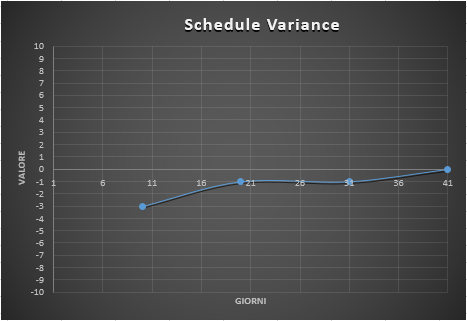
\includegraphics[scale=0.7]{Sezioni/Immagini/ScheduleVariance-RR}
	\caption{Schedule variance - RR}
\end{figure}

\begin{figure}[H]
	\centering 
	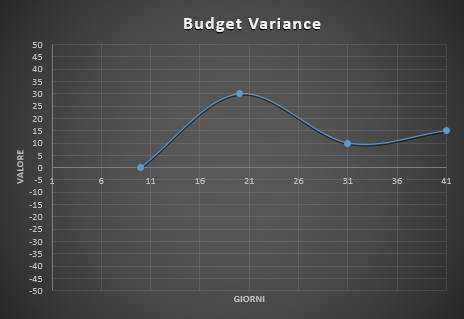
\includegraphics[scale=0.7]{Sezioni/Immagini/BudgetVariance-RR}
	\caption{Budget variance - RR}
\end{figure}

\subsubsection{Livello dei processi}
\begin{longtable}{|>{\centering}m{6cm}|c|c|c|c|c|}
\hline
\textbf{Processo} & \textbf{Livello} & \textbf{Esito} & \textbf{Valore}\\
\hline
\endhead
\emph{Processo di fornitura} & \textcolor{Green}{1} & Superato & Accettabile\\ \hline
\emph{Processo di sviluppo} & \textcolor{Green}{2}* & Superato & Accettabile\\ \hline
\emph{Processo di documentazione} & \textcolor{Green}{2} & Superato & Accettabile\\ 
\hline
\emph{Processo di Configurazione} & \textcolor{Green}{1} & Superato & Ottimale\\ 
\hline
\emph{Processo di garanzia di qualità del Prodotto} & * & / & /\\ 
\hline
\emph{Processo di Verifica} & \textcolor{Green}{1} & Superato & Ottimale\\ 
\hline
\emph{Processo di Validazione} & * & / & /\\ 
\hline
\emph{Processo di Risoluzione dei problemi} & \textcolor{Green}{1} & Superato & Ottimale\\ 
\hline
\emph{Processo di Coordinamento} & \textcolor{Green}{1} & Superato & Ottimale\\ 
\hline
\emph{Processo di Pianificazione} & \textcolor{Green}{1} & Superato & Ottimale\\ 
\hline
\emph{Processo di Formazione} & \textcolor{Green}{1} & Superato & Ottimale\\ 
\hline
\caption{RR-Livello dei processi}
\end{longtable}

Per i processi con segnatura \texttt{Voto*} vengono considerate solo le attività inerenti al lavoro che deve essere svolto per la \textit{Revisione di progettazione}. Per quelli, invece, con solo \texttt{*} significa che nessuna attività di quel processo era necessaria per il raggiungimento della milestone esterna.

\newpage

\subsection{Revisione di Progettazione}

\subsubsection{Analisi statica dei documenti}
L'analisi statica dei documenti è stata fatta mediante \termine{Walkthrough} ed ha portato all'individuazione di alcuni errori. Tra gli errori individuati quelli più frequenti sono stati:
		\begin{itemize}
			\item Errori ortografici.
			\item Parole con lettere mancanti o invertite.
			\item Periodi troppo lunghi o complessi da capire ed interpretare.
		\end{itemize}

\subsection{Metriche per i documenti}

\subsubsection{Indice di Gulpease}

\begin{table}[h]
	\begin{center}
		\begin{tabular}{|c|c|c|c|c|}
			\hline
			\textbf{Documento}	& \textbf{Risultato} & \textbf{Esito} & \textbf{Valore}\\
			\hline
		 \termine{Analisi} dei Requisiti v2.0.0 &	90 & Superato & Ottimale\\
			\hline
			Glossario v2.0.0 &	54 & Superato & Ottimale\\
			\hline
			Norme di Progetto v2.0.0 &	52 & Superato & Ottimale\\
			\hline
			Piano di Progetto v2.0.0	&	52 & Superato & Ottimale\\
			\hline
			Piano di Qualifica v2.0.0	&	46 & Superato & Accettabile\\
			\hline
			Definizione di \termine{Prodotto} v1.0.0	&	64 & Superato & Ottimale\\
			\hline
			Verbale\_Interno\_2\_20170222 v1.0.0	&	54 & Superato & Ottimale\\
			\hline
			Verbale\_Esterno\_3\_20170224 v1.0.0	&	53 & Superato & Ottimale\\
			\hline
			Verbale\_Interno\_4\_20170226 v1.0.0	&	51 & Superato & Ottimale\\
			\hline
			Verbale\_Interno\_5\_20170228 v1.0.0	&	52 & Superato & Ottimale\\
			\hline
		\end{tabular}
	\end{center}
	\caption{RP - Risultato indice di Gulpease}
\end{table}

\subsubsection{Soddisfacimento metriche}

\paragraph{Qualità di processo}
\begin{longtable}{|>{\centering}m{5cm}|c|c|c|c|c|}
\hline
\textbf{Metrica} & \textbf{Unità di misura} & \textbf{Risultato} & \textbf{Risultato Massimo} & \textbf{Esito} & \textbf{Valore}\\
\hline
\endhead

\emph{Schedule Variance} & {Attività} & \textcolor{Green}{0} & / & Superato & Ottimale\\ \hline
\emph{Budget Variance} & {Euro} & \textcolor{Orange}{-50} & / & Non superato & /\\ \hline
\emph{Ottimalità delle misurazioni} & {Percentuale} & \textcolor{Green}{0.6} & / & Superato & Ottimale \\ \hline
\emph{Rischi non preventivati} & {Rischi} & \textcolor{Green}{2} & / & Superato & Accettabile\\ \hline
%\emph{Efficienza di gestione dei rischi} & {Giorni} & \textcolor{Orange}{21.3} & $\geq 20$ & $\geq 60$\\ \hline
%\emph{Requisiti obbligatori soddisfatti} & {Percentuale} & \textcolor{Green}{100} & $100$ & $100$\\ \hline
\emph{Livello di instabilità-SDK} & {Percentuale} & / &\textcolor{Green}{1} & Superato & Accettabile\\ \hline
\emph{Livello di instabilità-Applicazione} & {Percentuale} & / &\textcolor{Green}{1} & Superato & Accettabile\\ \hline
\emph{Astrattezza-SDK} & {Percentuale} & \textcolor{Green}{0.8} & / & Superato & Accettabile\\ \hline
\emph{Astrattezza-Applicazione} & {Percentuale} & \textcolor{Green}{0.5} & / & Superato & Ottimale\\ \hline
\emph{Distanza dalla sequenza principale-SDK} & {Percentuale} & / &\textcolor{Green}{1} & Superato & Accettabile\\ \hline
\emph{Distanza dalla sequenza principale-Applicazione} & {Percentuale} & / &\textcolor{Green}{0.7} & Superato & Accettabile\\ \hline
\emph{Numero di metodi per classe} & {Metodi} & / &\textcolor{Green}{11} & Superato & Accettabile\\ \hline
\emph{Numero di attributi per classe} & {Attributi} & / &\textcolor{Green}{7} & Superato & Ottimale\\ \hline
\emph{Numero di parametri per metodo} & {Parametri} & / &\textcolor{Green}{7} & Superato & Ottimale\\ \hline
%\emph{Produttività di codifica} & {Linee} & \textcolor{Orange}{9.1} & $\geq 3$ & $\geq 10$\\ \hline
%\emph{Complessità Ciclomatica media} & {Cammini} & \textcolor{Green}{0} & $1 - 15$ & $1 - 10$\\ \hline
%\emph{Livelli di annidamento medi} & {Chiamate} & \textcolor{Green}{1} & $1 - 6$ & $1 - 3$\\ \hline
%\emph{Linee di codice per linee di commento} & {Percentuale} & \textcolor{Green}{31} & $\geq 25$ & $\geq 30$\\ \hline
%\emph{Variabili inutilizzate} & {Variabili} & \textcolor{Green}{0} & $0$ & $0$\\ \hline
%\emph{Dipendenze} & {Chiamate require} & \textcolor{Green}{2.2} & $0 - 10$ & $0 - 5$\\ \hline
%\emph{Halstead Difficulty media} & {Percentuale} & \textcolor{Green}{0} & $0 - 25$ & $0 - 15$\\ \hline
%\emph{Halstead Volume media} & {Percentuale} & \textcolor{Green}{20} & $20 - 1500$ & $20 - 1000$\\ \hline
%\emph{Halstead Effort media} & {Percentuale} & \textcolor{Green}{0} & $0 - 400$ & $0 - 300$\\ \hline
%\emph{Indice di manutenibilità} & {Percentuale} & \textcolor{Orange}{5.14} & $100 - 171$ & $120 - 171$\\ \hline
%\emph{Componenti integrate} & {Percentuale} & \textcolor{Green}{100} & $100$ & $100$\\ \hline
%\emph{Test di Unità eseguiti} & {Percentuale} & \textcolor{Red}{36.6} & $90 - 100$ & $100$\\ \hline
%\emph{Test di Integrazione eseguiti} & {Percentuale} & \textcolor{Red}{0} & $60 - 100$ & $70 - 100$\\ \hline
%\emph{Test di Sistema eseguiti} & {Percentuale} & \textcolor{Red}{0} & $70 - 100$ & $80 - 100$\\ \hline
%\emph{Test di \termine{Validazione} eseguiti} & {Percentuale} & \textcolor{Red}{0} & $100$ & $100$\\ \hline
%\emph{Test superati} & {Percentuale} & \textcolor{Green}{100} & $90 - 100$ & $100$\\ \hline
%\emph{Branch Coverage} & {Percentuale} & \textcolor{Orange}{73.3} & $70 - 100$ & $80 - 100$\\ \hline
%\emph{Code Coverage} & {Percentuale} & \textcolor{Green}{76.57} & $60 - 100$ & $70 - 100$\\ \hline
\caption{RP-Metriche di qualità di processo}
\end{longtable}

\subsubsection{Esiti delle metriche ripetute nel tempo}

\begin{figure}[H]
	\centering 
	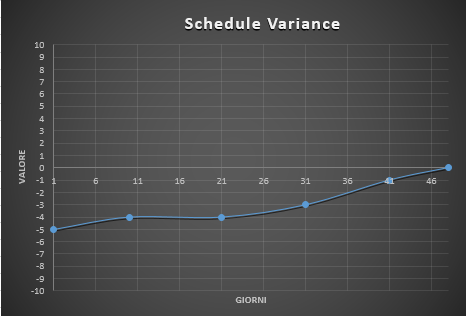
\includegraphics[scale=0.7]{Sezioni/Immagini/ScheduleVariance-RP}
	\caption{Schedule variance - RP}
\end{figure}

\begin{figure}[H]
	\centering 
	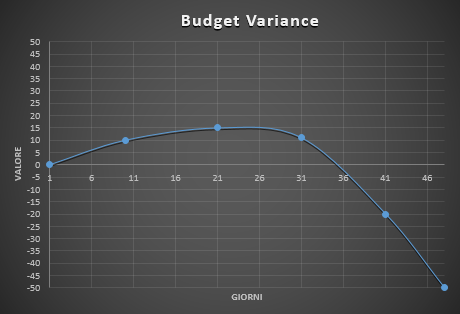
\includegraphics[scale=0.7]{Sezioni/Immagini/BudgetVariance-RP}
	\caption{Budget variance - RP}
\end{figure}

\begin{figure}[H]
	\centering 
	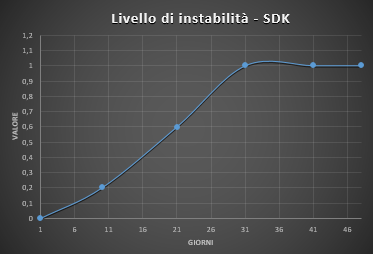
\includegraphics[scale=0.85]{Sezioni/Immagini/LivelloInstabilitaSDK-RP}
	\caption{Livello di instabilità SDK - RP}
\end{figure}

\begin{figure}[H]
	\centering 
	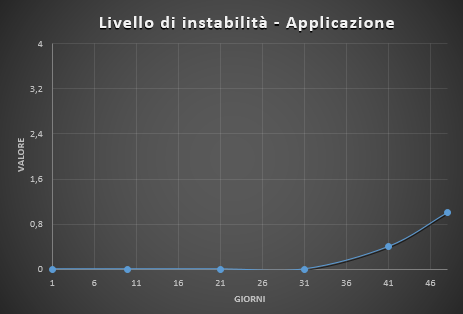
\includegraphics[scale=0.85]{Sezioni/Immagini/LivelloInstabilitaApp-RP}
	\caption{Livello di instabilità Applicazione - RP}
\end{figure}

\begin{figure}[H]
	\centering 
	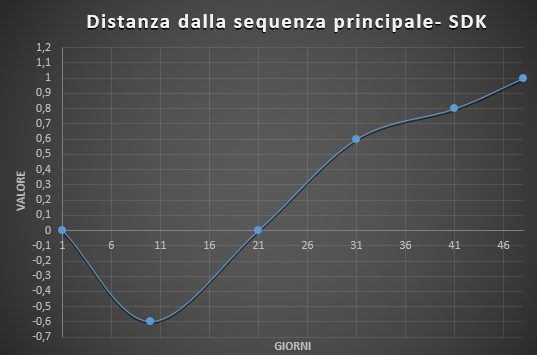
\includegraphics[scale=0.63]{Sezioni/Immagini/DistanzaSDK-RP}
	\caption{Distanza dalla sequenza principale SDK - RP}
\end{figure}

\begin{figure}[H]
	\centering 
	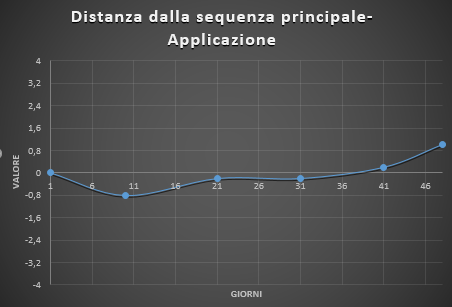
\includegraphics[scale=0.63]{Sezioni/Immagini/DistanzaApp-RP}
	\caption{Distanza dalla sequenza principale Applicazione - RP}
\end{figure}

\subsubsection{Livello dei processi}
\begin{longtable}{|>{\centering}m{6cm}|c|c|c|c|c|}
\hline
\textbf{Processo} & \textbf{Livello} & \textbf{Esito} & \textbf{Valore}\\
\hline
\endhead
\emph{Processo di fornitura} & \textcolor{Green}{2} & Superato & Ottimale\\ \hline
\emph{Processo di sviluppo} & \textcolor{Green}{2}* & Superato & Accettabile\\ \hline
\emph{Processo di documentazione} & \textcolor{Green}{2} & Superato & Accettabile\\ 
\hline
\emph{Processo di Configurazione} & \textcolor{Green}{1} & Superato & Ottimale\\ 
\hline
\emph{Processo di garanzia di qualità del Prodotto} & * & / & /\\ 
\hline
\emph{Processo di Verifica} & \textcolor{Green}{1} & Superato & Ottimale\\ 
\hline
\emph{Processo di Validazione} & * & / & /\\ 
\hline
\emph{Processo di Risoluzione dei problemi} & \textcolor{Green}{1} & Superato & Ottimale\\ 
\hline
\emph{Processo di Coordinamento} & \textcolor{Green}{1} & Superato & Ottimale\\ 
\hline
\emph{Processo di Pianificazione} & \textcolor{Green}{1} & Superato & Ottimale\\ 
\hline
\emph{Processo di Formazione} & \textcolor{Green}{1} & Superato & Ottimale\\ 
\hline
\caption{RP-Livello dei processi}
\end{longtable}

Per i processi con segnatura \texttt{Voto*} vengono considerate solo le attività inerenti al lavoro che deve essere svolto per la \textit{Revisione di progettazione}. Per quelli, invece, con solo \texttt{*} significa che nessuna attività di quel processo era necessaria per il raggiungimento della milestone esterna.

\newpage

\subsection{Revisione di Qualifica}

\subsubsection{Analisi statica dei documenti}
L'analisi statica dei documenti è stata fatta mediante \termine{Walkthrough} ed ha portato all'individuazione di alcuni errori. Tra gli errori individuati quelli più frequenti sono stati:
		\begin{itemize}
			\item Errori ortografici.
			\item Frasi complesse con un basso indice di comprensibilità.
		\end{itemize}

\subsection{Metriche per i documenti}

\subsubsection{Indice di Gulpease}

\begin{table}[h]
	\begin{center}
		\begin{tabular}{|c|c|c|c|c|}
			\hline
			\textbf{Documento}	& \textbf{Risultato} & \textbf{Esito} & \textbf{Valore}\\
			\hline
		    \termine{Analisi} dei Requisiti v3.0.0 & 87 & Superato & Ottimale\\
			\hline
			Glossario v3.0.0 & 55 & Superato & Ottimale\\
			\hline
			Norme di Progetto v3.0.0 & 46 & Superato & Accettabile\\
			\hline
			Piano di Progetto v3.0.0 & 48 & Superato & Accettabile\\
			\hline
			Piano di Qualifica v3.0.0 & 40 & Superato & Accettabile\\
			\hline
		 \termine{Manuale Utente} \termine{Monolith} v1.0.0 & 93 & Superato & Ottimale\\
			\hline
		 \termine{Manuale Utente} Bringit v1.0.0 & 48 & Superato & Accettabile\\
            \hline
            Verbale\_Interno\_7\_20170327 v1.0.0 & 67 & Superato & Ottimale\\
            \hline
            Verbale\_Interno\_8\_20170402 v1.0.0 & 73 & Superato & Ottimale\\
            \hline
            Verbale\_Interno\_9\_20170407 v1.0.0 & 78 & Superato & Ottimale\\
            \hline
            Verbale\_Esterno\_10\_20170503 v1.0.0 & 73 & Superato & Ottimale\\
            \hline
		\end{tabular}
	\end{center}
	\caption{RQ - Risultato indice di Gulpease}
\end{table}


\subsubsection{Soddisfacimento metriche}
\small{
Si noti che alcune componenti e i test a loro correlati non sono ancora state sviluppate, e che la loro assenza peserà nelle misurazioni.}

\paragraph{Qualità di processo}
\begin{longtable}{|>{\centering}m{5cm}|c|c|c|c|c|}
\hline
\textbf{Metrica} & \textbf{Unità di misura} & \textbf{Risultato} & \textbf{Risultato massimo} & \textbf{Esito} & \textbf{Valore}\\
\hline
\endhead
\emph{Schedule Variance} & {Attività} & \textcolor{Green}{0} & / & Superato & Ottimale\\ \hline
\emph{Budget Variance} & {Euro} & \textcolor{Orange}{-697} & / & Non superato & /\\ \hline
\emph{Ottimalità delle misurazioni} & {Percentuale} & \textcolor{Green}{74\%} & / & Superato & Ottimale \\ \hline
\emph{Rischi non preventivati} & {Rischi} & \textcolor{Green}{2} & / & Superato & Accettabile\\ \hline
\emph{Requisiti obbligatori soddisfatti} & {Percentuale} & \textcolor{Orange}{97.6\%} & / & Non superato & /\\ \hline
\emph{Livello di instabilità-SDK} & {Percentuale} & / & \textcolor{Green}{55\%} & Superato & Ottimale\\ \hline
\emph{Livello di instabilità-Applicazione} & {Percentuale} & / & \textcolor{Green}{70\%} & Superato & Accettabile\\ \hline
\emph{Astrattezza-SDK} & {Percentuale} & \textcolor{Green}{20\%} & / & Superato & Ottimale\\ \hline
\emph{Astrattezza-Applicazione} & {Percentuale} &\textcolor{Green}{15\%} & / & Superato & Ottimale\\ \hline
\emph{Distanza dalla sequenza principale-SDK} & {Percentuale} & / & \textcolor{Green}{25\%} & Superato & Ottimale\\ \hline
\emph{Distanza dalla sequenza principale-Applicazione} & {Percentuale} & / & \textcolor{Green}{15\%} & Superato & Ottimale\\ \hline
\emph{Numero di metodi per classe (max)} & {Metodi} & / & \textcolor{Green}{12} & Superato & Accettabile\\ \hline
\emph{Numero di attributi per classe (max)} & {Attributi} & / & \textcolor{Green}{7} & Superato & Ottimale\\ \hline
\emph{Numero di parametri per metodo (max)} & {Parametri} & / & \textcolor{Green}{5} & Superato & Ottimale\\ \hline
\emph{Complessità Ciclomatica media} & {Cammini} & \textcolor{Green}{1.3} & / & Superato & Ottimale\\ \hline
\emph{Livelli di annidamento medi} & {Chiamate} & \textcolor{Green}{2.4} & / & Superato & Ottimale\\ \hline
\emph{Linee di codice per linee di commento - Monolith} & {Percentuale} & \textcolor{Green}{28.3\%} & / & Superato & Ottimale\\ \hline
\emph{Linee di codice per linee di commento - BringIt} & {Percentuale} & \textcolor{Green}{20.5\%} & / & Superato & Ottimale\\ \hline
\emph{Componenti integrate} & {Percentuale} & \textcolor{Orange}{82\%} & / & Non superato & /\\ \hline
\emph{Test di Unità eseguiti} & {Percentuale} & \textcolor{Green}{99\%} & / & Superato & Ottimale\\ \hline
\emph{Test di Integrazione eseguiti} & {Percentuale} & \textcolor{Green}{84.7\%} & / & Superato & Ottimale\\ \hline
\emph{Test di Sistema eseguiti} & {Percentuale} & \textcolor{Green}{86\%} & / & Superato & Ottimale\\ \hline
\emph{Test di \termine{Validazione} eseguiti} & {Percentuale} & \textcolor{Orange}{46\%} & / & Non superato & / \\ \hline
\emph{Test superati} & {Percentuale} & \textcolor{Green}{100\%} & / & Superato & Ottimale \\ \hline
\emph{Branch Coverage} & {Percentuale} & \textcolor{Green}{83\%} & / & Superato & Accettabile\\ \hline
\emph{Statement Coverage} & {Percentuale} & \textcolor{Green}{77.4\%} & / & Superato & Accettabile\\ \hline
\emph{Accuratezza rispetto alle attese} & {Percentuale} & \textcolor{Green}{100} & / & Superato & Ottimale\\ \hline
\emph{Completezza dell’implementazione funzionale} & {Percentuale} & \textcolor{Orange}{86} & / & Non superato & /\\ \hline
\emph{Densità di failure} & {Percentuale} & \textcolor{Green}{0} & / & Superato & Ottimale\\ \hline
\emph{Blocco di operazioni non corrette} & {Percentuale} & \textcolor{Green}{90} & / & Superato & Accettabile\\ \hline
\emph{Tempo di risposta} & {Secondi} & / & \textcolor{Green}{1.0} & Superato & Ottimale\\ \hline
\emph{Capacità di analisi di failure} & {Percentuale} & \textcolor{Green}{100} & / & Superato & Ottimale\\ \hline
\emph{Impatto delle modifiche} & {Indice} & \textcolor{Green}{2} & / & Superato & Ottimale\\ \hline
\caption{RQ-Metriche di qualità di processo}\\
\end{longtable}

\subsubsection{Esiti delle metriche ripetute nel tempo}

\begin{figure}[H]
	\centering 
	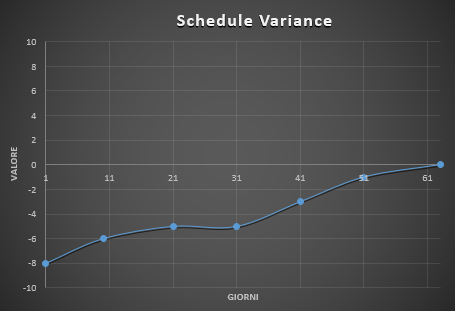
\includegraphics[scale=0.7]{Sezioni/Immagini/ScheduleVariance-RQ}
	\caption{Schedule variance - RQ}
\end{figure}

\begin{figure}[H]
	\centering 
	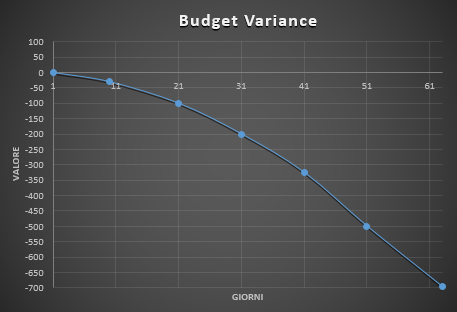
\includegraphics[scale=0.7]{Sezioni/Immagini/BudgetVariance-RQ}
	\caption{Budget variance - RQ}
\end{figure}

\begin{figure}[H]
	\centering 
	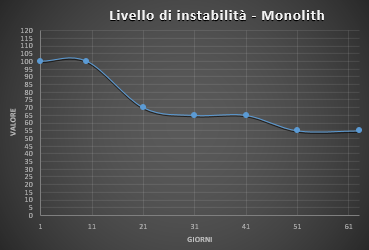
\includegraphics[scale=0.85]{Sezioni/Immagini/LivelloInstabilitaSDK-RQ}
	\caption{Livello di instabilità Monolith - RQ}
\end{figure}

\begin{figure}[H]
	\centering 
	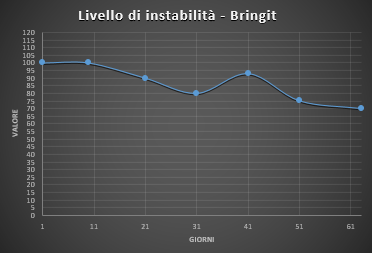
\includegraphics[scale=0.85]{Sezioni/Immagini/LivelloInstabilitaApp-RQ}
	\caption{Livello di instabilità Bringit - RQ}
\end{figure}

\begin{figure}[H]
	\centering 
	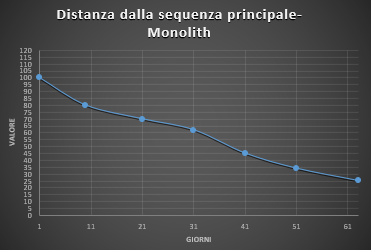
\includegraphics[scale=0.85]{Sezioni/Immagini/DistanzaSDK-RQ}
	\caption{Distanza dalla sequenza principale Monolith - RQ}
\end{figure}

\begin{figure}[H]
	\centering 
	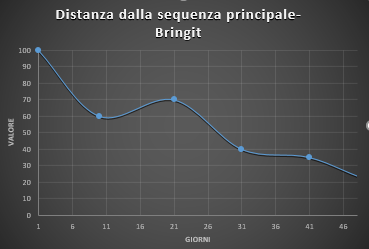
\includegraphics[scale=0.85]{Sezioni/Immagini/DistanzaApp-RQ}
	\caption{Distanza dalla sequenza principale Bringit - RQ}
\end{figure}

\begin{figure}[H]
	\centering 
	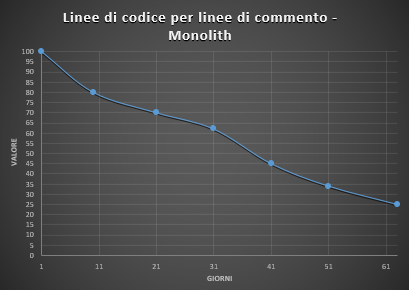
\includegraphics[scale=0.8]{Sezioni/Immagini/LineeCodiceCommentoSDK-RQ}
	\caption{Linee di codice per linee di commento Monolith - RQ}
\end{figure}

\begin{figure}[H]
	\centering 
	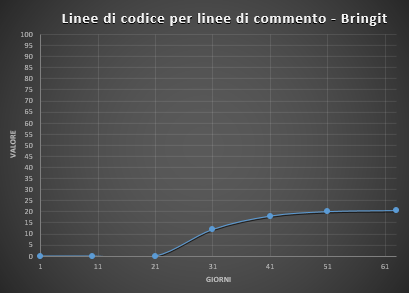
\includegraphics[scale=0.8]{Sezioni/Immagini/LineeCodiceCommentoApp-RQ}
	\caption{Linee di codice per linee di commento Bringit - RQ}
\end{figure}

\subsubsection{Livello dei processi}
\begin{longtable}{|>{\centering}m{6cm}|c|c|c|c|c|}
\hline
\textbf{Processo} & \textbf{Livello} & \textbf{Esito} & \textbf{Valore}\\
\hline
\endhead
\emph{Processo di fornitura} & \textcolor{Green}{2} & Superato & Ottimale\\ \hline
\emph{Processo di sviluppo} & \textcolor{Green}{2}* & Superato & Accettabile\\ \hline
\emph{Processo di documentazione} & \textcolor{Green}{2} & Superato & Accettabile\\ 
\hline
\emph{Processo di Configurazione} & \textcolor{Green}{1} & Superato & Ottimale\\ 
\hline
\emph{Processo di garanzia di qualità del Prodotto} & * & / & /\\ 
\hline
\emph{Processo di Verifica} & \textcolor{Green}{1} & Superato & Ottimale\\ 
\hline
\emph{Processo di Validazione} & * & / & /\\ 
\hline
\emph{Processo di Risoluzione dei problemi} & \textcolor{Green}{1} & Superato & Ottimale\\ 
\hline
\emph{Processo di Coordinamento} & \textcolor{Green}{1} & Superato & Ottimale\\ 
\hline
\emph{Processo di Pianificazione} & \textcolor{Green}{1} & Superato & Ottimale\\ 
\hline
\emph{Processo di Formazione} & \textcolor{Green}{1} & Superato & Ottimale\\ 
\hline
\caption{RQ-Livello dei processi}
\end{longtable}
\newpage

\subsubsection{Esito dei test di unità}
\begin{center}
	\begin{longtable}{|c|>{\centering}m{10cm}|c|}\hline
		Id & Descrizione & Esito\\ \hline
		TU1 & Verificare che in un widget di tipo testo venga impostata in modo corretto la grandezza del font del testo & \textcolor{Green}{Superato}\\ \hline
		TU2 & Verificare che all'instanziazione di un widget di tipo testo la grandezza del testo sia di default a 1em & \textcolor{Green}{Superato}\\ \hline
		TU3 & Verificare che all'interno di un widget di tipo testo venga impostata in corsivo la parte di testo richiesta & \textcolor{Green}{Superato}\\ \hline
		TU4 & Verificare che all'interno di un widget di tipo testo venga inserito un link cliccabile nel modo corretto & \textcolor{Green}{Superato}\\ \hline
		TU5 & Verificare che all'interno di un widget di tipo testo i link cliccabili abbiano il colore corretto & \textcolor{Green}{Superato}\\ \hline
		TU6 & Verificare che all'interno di un widget di tipo testo venga impostata in grassetto la parte di testo richiesta & \textcolor{Green}{Superato}\\ \hline
		TU7 & Verificare che all'interno di un widget di tipo testo venga impostato il colore del testo in modo corretto & \textcolor{Green}{Superato}\\ \hline
		TU8 & Verificare che all'instanziazione di un widget di tipo testo il colore del testo sia di default a nero & \textcolor{Green}{Superato}\\ \hline
		TU9 & Verificare che in un widget di tipo immagine l'immagine venga agiunta in modo corretto & \textcolor{Green}{Superato}\\ \hline
		TU10 & Verificare che in un widget di tipo immagine venga mostrato il messaggio di errore appropriato nel caso si inserisca un immagina non valida & \textcolor{Green}{Superato}\\ \hline
		TU11 & Verificare che un widget di tipo immagine venga impostata la dimensione del immagine da visualizzare in modo corretto & \textcolor{Green}{Superato}\\ \hline
		TU12 & Verificare che all'instanziazione di un widget di tipo immagine venga impostata la larghezza e l'altezza di default & \textcolor{Green}{Superato}\\ \hline
		TU13 & Verificare un widget di tipo immagine venga visualizzato con le dimensioni corrette & \textcolor{Green}{Superato}\\ \hline
		TU14 & Verificare che in un widget di tipo bottone venga impostato il testo in modo corretto & \textcolor{Green}{Superato}\\ \hline
		TU15 & Verificare che venga mostrarto in modo corretto il messaggio di errore se viene inserita una sequenza di caratteri non valida in un widget di tipo bottone & \textcolor{Green}{Superato}\\ \hline
		TU16 & Verificare che un widget di tipo bottone venga impostata la dimensione in modo corretto & \textcolor{Green}{Superato}\\ \hline
		TU17 & Verificare che all'instanziazione di un widget di tipo bottone venga impostata la larghezza e l'altezza di default & \textcolor{Green}{Superato}\\ \hline
		TU18 & Verificare che in un widget di tipo bottone venga impostato il colore di sfondo in modo corretto & \textcolor{Green}{Superato}\\ \hline
		TU19 & Verificare che all'instanziazione di un widget di tipo bottone venga impostato il colore di sfondo di default & \textcolor{Green}{Superato}\\ \hline
		TU20 & Verificare che in un widget di tipo button vengano eseguiti gli eventi associati alla pressione & \textcolor{Green}{Superato}\\ \hline
		TU21 & Verificare che in un widget di tipo button vengano eseguiti gli eventi associati alla pressione pressione prolungata & \textcolor{Green}{Superato}\\ \hline
		TU22 & Verificare che in un widget di tipo button venga impostato in modo corretto la soglia per determinare che una pressione da parte del utente è di tipo: "pressione prolungata" & \textcolor{Green}{Superato}\\ \hline
		TU23 & Verificare che un un widget di tipo checklistitem venga cambiato in modo corretto la stato da "cliccato" a "non cliccato" e viceversa & \textcolor{Green}{Superato}\\ \hline
		TU24 & Verificare che all'instanziazione di un widget di tipo checklistitem venga impostato lo stato a "non cliccato" & \textcolor{Green}{Superato}\\ \hline
		TU25 & Verificare che un widget di tipo checklistitem venga visualizzato con lo stile di spunta e colore corretto & \textcolor{Green}{Superato}\\ \hline
		TU26 & Verificare che in un widget di tipo checklistitem vengano associati gli eventi di pressione nel modo corretto & \textcolor{Green}{Superato}\\ \hline
		TU27 & Verificare che in un widget di tipo checklistitem vengano associati gli eventi di pressione prolungata nel modo corretto & \textcolor{Green}{Superato}\\ \hline
		TU28 & Verificare che in un widget di tipo checklistitem vengano eseguiti gli eventi associati alla pressione & \textcolor{Green}{Superato}\\ \hline
		TU29 & Verificare che in un widget di tipo checklistitem vengano eseguiti gli eventi associati alla pressione pressione prolungata & \textcolor{Green}{Superato}\\ \hline
		TU30 & Verificare che in un widget di tipo checklistitem venga impostato in modo corretto la soglia per determinare che una pressione da parte del utente è di tipo: "pressione prolungata" & \textcolor{Green}{Superato}\\ \hline
		TU31 & Verificare che in un widget di tipo list venga impostato correttamente il cambiamento dell'indicatore a 'pallino' & \textcolor{Green}{Superato}\\ \hline
		TU32 & Verificare che in un widget di tipo list venga impostato correttamente il cambiamento dell'indicatore a 'trattino' & \textcolor{Green}{Superato}\\ \hline
		TU33 & Verificare che in un widget di tipo list venga impostato correttamente il cambiamento dell'indicatore ad elenco numerato & \textcolor{Green}{Superato}\\ \hline
		TU34 & Verificare che in un widget di tipo list che vengano aggiunti correttamente tutti gli elementi & \textcolor{Green}{Superato}\\ \hline
		TU35 & Verificare che in un layout verticale sia possibile aggiungere un elemento & \textcolor{Green}{Superato}\\ \hline
		TU36 & Verificare che in un layout verticale non sia possibile aggiungere se stesso & \textcolor{Green}{Superato}\\ \hline
		TU37 & Verificare che in un layout orizzontale sia possibile aggiungere un elemento & \textcolor{Green}{Superato}\\ \hline
		TU38 & Verificare che in un layout orizzontale non sia possibile aggiungere se stesso & \textcolor{Green}{Superato}\\ \hline
		TU39 & Verificare che il nome della lista della spesa venga impostato nel modo corretto & \textcolor{Green}{Superato}\\ \hline
		TU40 & Verificare che all'instanziazione di una lista della spesa venga impostato il valore di default per il nome della lista & \textcolor{Green}{Superato}\\ \hline
		TU41 & Verificare che nel caso di un errore durante l'aggiunta di un prodotto alla lista della spesa venga mostrato un mesaggio di errore & \textcolor{Green}{Superato}\\ \hline
		TU42 & Verificare che l'immagine del prodotto venga aggiunta in modo corretto & \textcolor{Green}{Superato}\\ \hline
		TU43 & Verificare che la descrizione del prodotto venga aggiunta in modo corretto & \textcolor{Green}{Superato}\\ \hline
		TU44 & Verificare che le note del prodotto vengano aggiunte in modo corretto & \textcolor{Orange}{Non superato}\\ \hline
		TU45 & Verificare che la quantità del prodotto venga impostata in modo corretto quando inserita & \textcolor{Green}{Superato}\\ \hline
		TU46 & Verificare che alla creazione di un nuovo prodotto venga impostata la quantità di default & \textcolor{Green}{Superato}\\ \hline
		TU47 & Verificare che l'unità di misura relativa alla quantità del prodotto venga impostata in modo corretto & \textcolor{Green}{Superato}\\ \hline
		TU48 & Verificare che alla creazione di un nuovo prodotto venga impostata l'unità di misura di default & \textcolor{Green}{Superato}\\ \hline
		TU49 & Verificare che DatabaseSource ritorni la lista che corrisponde all'id inserito & \textcolor{Green}{Superato}\\ \hline
		TU50 & Verificare che DatabaseSource ritorni l'oggetto che corrisponde all'id inserito & \textcolor{Green}{Superato}\\ \hline
		TU51 & Verificare che DatabaseSource cancelli la lista che corrisponde all'id inserito & \textcolor{Green}{Superato}\\ \hline
		TU52 & Verificare che DatabaseSource salvi correttamente la lista nel database & \textcolor{Green}{Superato}\\ \hline
		TU53 & Verificare che ModifyListUseCase aggiunga correttamente un item alla lista nel database & \textcolor{Green}{Superato}\\ \hline
		TU54 & Verificare che ModifyListUseCase rimuova correttamente un item alla lista nel database & \textcolor{Green}{Superato}\\ \hline
		TU55 & Verificare che ModifyListUseCase aggiorni correttamente un item alla lista nel database & \textcolor{Green}{Superato}\\ \hline
		TU56 & Verificare che DeleteListViewPresenter funzioni correttamente senza lanciare eccezioni & \textcolor{Green}{Superato}\\ \hline
		TU57 & Verificare che InputListInfoViewPresenter crei correttamente un elemento della lista & \textcolor{Green}{Superato}\\ \hline
		TU58 & Verificare che ShareWithGroupViewPresenter funzioni correttamente senza lanciare eccezioni & \textcolor{Green}{Superato}\\ \hline
		TU59 & Verificare che ShareWithContactViewPresenter funzioni correttamente senza lanciare eccezioni & \textcolor{Green}{Superato}\\ \hline
	\end{longtable}
\end{center}

\newpage

\subsubsection{Esito dei test di integrazione}
\begin{center}
	\begin{longtable}{|c|>{\centering}m{10cm}|c|}\hline
		Id & Descrizione & Esito\\ \hline
		TI1 & Si verifica che il metodo ButtonWidget::setText passi correttamente il testo al presenter il quale eventualmente lo formatterà e modificherà correttamente l'HTML e CSS & \textcolor{Green}{Superato}\\ \hline
		TI2 & Si verifica che il metodo ButtonWidget::setHeight passi correttamente il valore dell'altezza al presenter il quale modificherà correttamente l'HTML e CSS & \textcolor{Green}{Superato}\\ \hline
		TI3 & Si verifica che il metodo ButtonWidget::setWidth passi correttamente il valore della lareghezza al presenter modificherà correttamente l'HTML e CSS & \textcolor{Green}{Superato}\\ \hline
		TI4 & Si verifica che il metodo ButtonWidget::setBackgroundColor passi correttamente il colore dello sfondo del bottone al presenter il quale modificherà correttamente l'HTML e CSS & \textcolor{Green}{Superato}\\ \hline
		TI5 & Si verifica che il metodo ButtonWidget::setOnClickAction passi correttamente al presenter la funzione che verrà eseguita quanto viene premuto il pulsante & \textcolor{Green}{Superato}\\ \hline
		TI6 & Si verifica che il metodo ButtonWidget::setOnLongClickAction passi correttamente al presenter la funzione che verrà eseguita quanto viene mantenuto premuto il pulsante & \textcolor{Green}{Superato}\\ \hline
		TI7 & Si verifica che il metodo TextWidget::setText passi correttamente al presenter il testo che verrà poi mostrato a video & \textcolor{Green}{Superato}\\ \hline
		TI8 & Si verifica che il metodo TextWidget::setTextColor passi correttamente il colore del testo al presenter il quale modificherà correttamente l'HTML e CSS, presentandolo con il colore corrispondente & \textcolor{Green}{Superato}\\ \hline
		TI9 & Si verifica che il metodo TextWidget::setFormatText passi il valore booleano (che rappresenta la scelta di formattare il testo) al presenter. Esso dovrà, poi, presentare il testo formattato seguendo la sintassi markdown oppure lasciarlo invariato in funzione al valore booleano & \textcolor{Green}{Superato}\\ \hline
		TI10 & Si verifica che il metodo TextWidget::setUrlHighlightColor passi il valore del colore al presenter il quale dovrà presentare i link evidenziati oppure non evidenziati in funzione al colore scelto & \textcolor{Green}{Superato}\\ \hline
		TI11 & Si verifica che il metodo TextWidget::setTextSize passi la dimensione del testo del presenter il quale dovrà occuparsi di presentare il testo della dimensione impostata & \textcolor{Green}{Superato}\\ \hline
		TI12 & Si verifica che il metodo ChecklistItemWidget::setUseSelectionMark imposti la scelta di utilizzare un carattere o un colore come spunta passando correttamente per il Presenter & \textcolor{Green}{Superato}\\ \hline
		TI13 & Si verifica che il metodo ChecklistItemWidget::setSelectionColor passi al presenter il colore dello spunta il quale dovrà presentare la lista con lo stile corretto & \textcolor{Green}{Superato}\\ \hline
		TI14 & Si verifica che il metodo ChecklistItemWidget::setSelectionCharacter passi al presenter un carattere per la spunta, e il presenter dovrà presentare la lista con lo stile corretto & \textcolor{Green}{Superato}\\ \hline
		TI15 & Si verifica che il metodo ListWidget::addItem passi al presenter il testo del elemento il quale dovrà presentare l'HTML con il nuovo elemento & \textcolor{Green}{Superato}\\ \hline
		TI16 & Si verifica che la view passi al presenter il carattere con il quale mostrare gli indicatori della lista. Esso provvederà poi ad impostarli correttamente nell'HTML & \textcolor{Green}{Superato}\\ \hline
		TI17 & Si verifica che il metodo ImageWidget::setWidth passi correttamente al presenter il valore dell'altezza il quale aggiornerà la view & \textcolor{Green}{Superato}\\ \hline
		TI18 & Si verifica che il metodo ImageWidget::setHeight passi correttamente al presenter il valore della larghezza il quale aggiornerà la view & \textcolor{Green}{Superato}\\ \hline
		TI19 & Si verifica che il metodo ImageWidget::setImage passi correttamente al presenter il path del'immagine che dovrà essere presentata nella view & \textcolor{Green}{Superato}\\ \hline
		TI20 & Si verifica che l'aggiunta di un VerticalLayoutView, creato con degli elementi al suo interno, non causi errori nell'aggiunta di questo alla bolla e che, gli elementi, nel layout appena aggiunto, vengano mostrati uno sotto l'altro & \textcolor{Green}{Superato}\\ \hline
		TI21 & Si verifica che l'aggiunta di un HorizontalLayoutView, creato con degli elementi al suo interno, non causi errori nell'aggiunta di questi alla bolla e che gli elementi, nel layout appena aggiunto, vengano mostrati uno vicino all'altro & \textcolor{Green}{Superato}\\ \hline
		TI22 & Si verifica che il ModifyListUseCase esegua le operazioni di aggiunta, rimozione e aggiornamento dei dati trammite DatabaseSource in modo corretto & \textcolor{Green}{Superato}\\ \hline
		TI23 & Si verifica che ShareWithGroupViewPresenter interagisca in modo corretto con ChatSource & \textcolor{Green}{Superato}\\ \hline
		TI24 & Si verifica che CreateListViewPresenter interagisca con ChatSource in modo corretto & \textcolor{Green}{Superato}\\ \hline
		TI25 & Si verifica che ShareListUseCase interagisca in modo corretto con DatabaseSource & \textcolor{Green}{Superato}\\ \hline
		TI26 & Si verifica che ManageListUseCase interagisca con DatabaseSource rimuovendo e aggiungendo una lista dal database in modo corretto & \textcolor{Green}{Superato}\\ \hline
		TI27 & Si verifica che DeleteListViewPresenter interagisca con ShowPopupUseCase mostrando il popup di eliminazione della lista & \textcolor{Green}{Superato}\\ \hline
		TI28 & Si verifica che ForwardListUseCase interagisca in modo corretto con ChatSource al fine di inoltrare la lista selezionata & \textcolor{Orange}{Non superato}\\ \hline
		TI29 & Si verifica che GetListInfoUseCase esegua i fetch dei dati in modo corretto dal database tramite DatabaseSource & \textcolor{Green}{Superato}\\ \hline
		TI30 & Si verifica che ChangeListInfoViewPresenter interagisca in modo corretto con ModifyListUseCase & \textcolor{Orange}{Non superato}\\ \hline
		TI31 & Si verifica che ChangeListInfoViewPresenter interagisca in modo corretto con ShowPopupUseCase & \textcolor{Orange}{Non superato}\\ \hline
		TI32 & Si verifica che ShareWithGroupViewImpl interagisca in modo corretto con ShareWithGroupViewPresenter & \textcolor{Green}{Superato}\\ \hline
		TI33 & Si verifica che ShareWithContactViewImpl interagisca in modo corretto con ShareWithContactViewPresenter & \textcolor{Green}{Superato}\\ \hline
		TI34 & Si verifica che GetItemInfoUseCase interagisca in modo corretto con DatabaseSource & \textcolor{Green}{Superato}\\ \hline
		TI35 & Si verifica che ModifyItemPresenter interagisca in modod corretto con ModifyListUseCase & \textcolor{Orange}{Non superato}\\ \hline
		TI36 & Si verifica che ModifyItemPresenter interagisca in modod corretto con ShowPopupUseCase & \textcolor{Orange}{Non superato}\\ \hline
		TI37 & Si verifica che ModifyItemView interagisca in modod corretto con ModifyItemPresenter & \textcolor{Orange}{Non superato}\\ \hline
		TI38 & Si verifica che ModifyListUseCase interagisca in modo corretto con DatabaseSource & \textcolor{Green}{Superato}\\ \hline
		TI39 & Si verifica che ShareWithContactViewPresenter interagisca in modo corretto con ChatSource & \textcolor{Green}{Superato}\\ \hline
		TI40 & Si verifica che ShareWithContactViewPresenter interagisca in modo corretto con ShowPopupUseCase & \textcolor{Green}{Superato}\\ \hline
		TI41 & Si verifica che CreateListViewImpl interagisca in modo corretto con CreateListViewPresenter & \textcolor{Green}{Superato}\\ \hline
		TI42 & Si verifica che DeleteListViewImpl interagisca in modo corretto con DeleteListViewPresenter & \textcolor{Green}{Superato}\\ \hline
		TI43 & Si verifica che InputListInfoViewImpl interagisca in modo corretto con InputListInfoViewPresenter & \textcolor{Green}{Superato}\\ \hline
		TI44 & Si verifica che InputItemInfoViewImpl interagisca in modo corretto con InputItemInfoViewPresenter & \textcolor{Green}{Superato}\\ \hline
	\end{longtable}
\end{center}

\newpage

\subsubsection{Esito dei test di sistyema}
\begin{center}
	\begin{longtable}{|c|>{\centering}m{10cm}|c|}\hline
		Id & Descrizione & Esito\\ \hline
		TSFO1 & Si verifica che sia possibile creare e aggiungere ad una bolla un widget per tipo, tra quelli presenti nell'SDK & \textcolor{Green}{Superato}\\ \hline
		TSFO2 & Si verifica che sia possibile creare e aggiungere ad una bolla un layout per tipo, tra quelli presenti nell'SDK & \textcolor{Green}{Superato}\\ \hline
		TSFO3 & Si verifica che sia possibile impostare le variabili di un widget testo formattato & \textcolor{Green}{Superato}\\ \hline
		TSFO4 & Si verifica che un widget testo formattato faccia visualizzare un messaggio d'errore in caso venga impostata una sua variabile in maniera errata & \textcolor{Green}{Superato}\\ \hline
		TSFO5 & Si verifica che sia possibile impostare le variabili di un widget immagine & \textcolor{Green}{Superato}\\ \hline
		TSFO6 & Si verifica che un widget immagine faccia visualizzare un messaggio d'errore in caso venga impostata una sua variabile in maniera errata & \textcolor{Green}{Superato}\\ \hline
		TSFO7 & Si verifica che sia possibile impostare le variabili di un widget bottone & \textcolor{Green}{Superato}\\ \hline
		TSFO8 & Si verifica che un widget bottone faccia visualizzare un messaggio d'errore in caso venga impostata una sua variabile in maniera errata & \textcolor{Green}{Superato}\\ \hline
		TSFO9 & Si verifica che sia possibile impostare le variabili di un widget checklistitem & \textcolor{Green}{Superato}\\ \hline
		TSFO10 & Si verifica che un widget checklistitem faccia visualizzare un messaggio d'errore in caso venga impostata una sua variabile in maniera errata & \textcolor{Green}{Superato}\\ \hline
		TSFO11 & Si verifica che sia possibile impostare le variabili di un widget lista & \textcolor{Green}{Superato}\\ \hline
		TSFO12 & Si verifica che un widget lista faccia visualizzare un messaggio d'errore in caso venga impostata una sua variabile in maniera errata & \textcolor{Green}{Superato}\\ \hline
		TSFO13 & Si verifica che sia possibile aggiungere un widget all'interno di un VerticalLayoutView & \textcolor{Green}{Superato}\\ \hline
		TSFO14 & Si verifica che sia possibile aggiungere un widget all'interno di un HorizzontalLayoutView & \textcolor{Green}{Superato}\\ \hline
		TSFO15 & Si verifica che sia possibile istanziare una bolla avviso e sia possibile utilizzare tutti i suoi metodi & \textcolor{Green}{Superato}\\ \hline
		TSFO16 & Si verifica che sia possibile istanziare una bolla markdown e sia possibile utilizzare tutti i suoi metodi & \textcolor{Green}{Superato}\\ \hline
		TSFO17 & Si verifica che sia possibile istanziare una bolla lista e sia possibile utilizzare tutti i suoi metodi & \textcolor{Green}{Superato}\\ \hline
		TSFO18 & Si verifica che sia possibile creare una bolla "lista della spesa" & \textcolor{Green}{Superato}\\ \hline
		TSFO19 & Si verifica che l'aggiunta di un nuovo prodotto alla lista della spesa venga eseguita correttamente & \textcolor{Green}{Superato}\\ \hline
		TSFF20 & Si verifica che sia possibile rimuovere, per un utente con i permessi ed al creatore, un elemento ad una bolla "lista della spesa" & \textcolor{Green}{Superato}\\ \hline
		TSFO21 & Si verifica che sia possibile spuntare, per tutti gli utenti, un elemento di una bolla "lista della spesa" & \textcolor{Green}{Superato}\\ \hline
		TSFO22 & Si verifica che la pubblicazione a un utente di una bolla "lista della spesa" avvenga in modo corretto & \textcolor{Green}{Superato}\\ \hline
		TSFO23 & Si verifica che la pubblicazione a un gruppo di una bolla "lista della spesa" avvenga in modo corretto & \textcolor{Green}{Superato}\\ \hline
		TSFO24 & Si verifica che l'utente con i permessi possa aggiungere elementi alla lista & \textcolor{Green}{Superato}\\ \hline
		TSFO25 & Si verifica che l'utente senza i permessi non possa aggiungere elementi alla lista & \textcolor{Green}{Superato}\\ \hline
		TSFO26 & Si verifica che il creatore della lista possa aggiungere elementi alla lista & \textcolor{Green}{Superato}\\ \hline
	\end{longtable}
\end{center}

\newpage

\subsubsection{Esito dei test di validazione}
\begin{center}
	\begin{longtable}{|c|>{\centering}m{10cm}|c|}\hline
		Id & Descrizione & Esito\\ \hline
		TVFO1 & Si verifica che l'SDK sia utilizzabile dall'applicazione di demo & \textcolor{Green}{Superato}\\ \hline
		TVFO2 & Si verifica che sia possibile istanziare tutti i widget che sono inclusi nell'SDK & \textcolor{Green}{Superato}\\ \hline
		TVFO3 & Si verifica che sia possibile istanziare tutti i layout che sono inclusi nell'SDK & \textcolor{Green}{Superato}\\ \hline
		TVFO4 & Si verifica che sia possibile istanziare tutte le bolle che sono incluse nell'SDK & \textcolor{Green}{Superato}\\ \hline
		TVFO5 & Si verifica che sia possibile comporre una bolla personalizzata mediante widget e layout & \textcolor{Green}{Superato}\\ \hline
		TVFO6 & Si verifica che un generico utente possa creare un lista della spesa e pubblicarla all'interno di un canale Rockt.chat & \textcolor{Green}{Superato}\\ \hline
		TVFO7 & Si verifica che un generico utente possa creare un lista della spesa e pubblicarla ad un singolo utente avente un account sull'istanza Rocket.chat su cui è installata l'SDK & \textcolor{Orange}{Non superato}\\ \hline
		TVFO8 & Si verifica che, se un utente ha i permessi per interagire con una bolla, quest'ultima sia in grado di visualizzare gli elementi e di spuntarli & \textcolor{Orange}{Non superato}\\ \hline
		TVFO9 & Si verifica che, se un utente inoltra una lista della spesa, quest'ultima venga inoltrata in forma testuale bloccando quindi ogni forma di interazione con l'utente & \textcolor{Orange}{Non superato}\\ \hline
		TVVO10 & Si verifica che tutti i file che contengono codice scritto in JavaScript o coffescript passino i test di linting & \textcolor{Green}{Superato}\\ \hline
		TVVO11 & Si verifica che l'SDK si installi correttamente in una istanza di Rocket.chat, della quale viene fatto hosting su Heroku & \textcolor{Orange}{Non superato}\\ \hline
		TVFO12 & Si verifica che l'SDK funzioni con il browser Chrome versione >= 56 & \textcolor{Orange}{Non superato}\\ \hline
		TVFO13 & Si verifica che l'SDK funzioni con il browser Safari versione >= 10 & \textcolor{Orange}{Non superato}\\ \hline
		TVFO14 & Si verifica che l'SDK funzioni con il browser Opera versione >= 43 & \textcolor{Orange}{Non superato}\\ \hline
		TVFO15 & Si verifica che l'SDK funzioni con il browser Firefox versione >= 45 & \textcolor{Orange}{Non superato}\\ \hline
		TVFO16 & Si verifica che l'SDK funzioni con il browser Microsoft Edge versione >= 13 & \textcolor{Orange}{Non superato}\\ \hline
	\end{longtable}
\end{center}

\newpage
